\documentclass[UTF8]{ctexart}
%笔者信息
\title{mmWave学习笔记}
\author{李东豫  Powered by TI}
\date{\today}
%包引用
\usepackage{amsmath}
\usepackage{graphicx}
%页边距设置
\usepackage{geometry}
\geometry{papersize={210mm,297mm}}
\geometry{left=3cm,right=2.5cm,top=2.5cm,bottom=2.5cm}
\begin{document}
\maketitle
\tableofcontents
\section{概述}
mmWave雷达是近来使用在众多无人驾驶项目中用于建图、避障的高性能传感器,具有分辨率高,不受恶劣天气干扰,隐私性好(想想如果在洗手间安装一个摄像头监控会有多尴尬)的优点。由于Estello无人载具项目开发的需要,我们选择TI的IWR1443毫米波雷达作为载体进行相关学习。
\section{mmWave基础知识}
本节将关注mmWave雷达测量距离、角度、速度的原理进行介绍。
\subsection{什么是FMCW}
\paragraph{FMCW雷达}
的核心是一种称为线性调频脉冲(Chirp)的信号。线性调频脉冲是指雷达信号的频率随时间线性增长的正弦波:f=at,时域波形请见下图\\
{\centering 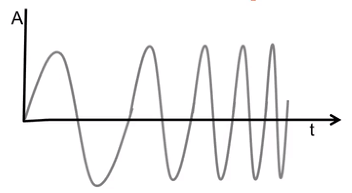
\includegraphics[width = .4\textwidth]{pic/FMCW.png}

}

假设线性调频脉冲以频率$f_c$开始,最终以$f_c+B$的频率结束,那么称B为线性调频脉冲的带宽。因此我们称其为调频连续波,即FMCW。下图为Chirp频域波形:

{\centering 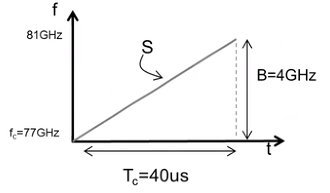
\includegraphics[width = .4\textwidth]{pic/FMCW_Fwave.png}

}

本图例即为IWR1443毫米波雷达的FMCW波形图,其FMCW由初始频率$f_c$,带宽B,以及持续时间$T_c$完全确定。其斜率S决定了线性调频脉冲的频率每单位时间增长的速率。可见在本图中,该线性调频脉冲在40us内扫过了4GHz的带宽,则斜率为100MHz/us.请注意:B和S为定义系统性能的重要参数。

\subsection{FMCW雷达测距原理}
\paragraph{1TX-1RX FMCW雷达}
前方的一个物体会产生一个中频信号(IF Signal)。设雷达信号从TX发射到RX天线接收的时间为τ,则$τ=2d/c$,c为光速,d为雷达与障碍物间距。由此产生的IF信号频率恒定,为$f_{IF}=Sτ=\frac{S2d}{c}.$可推测:雷达前方有多个距离不同的物体时,将产生多个IF信号。该IF信号的频率与距离成正比。

{\centering 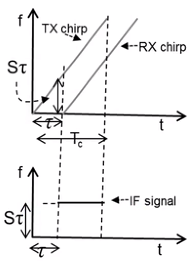
\includegraphics[width = .3\textwidth]{pic/TXRX.png}

}
\subsubsection{mmWave雷达的分辨率与探测距离}
主要是指傅里叶变换对多个距离不同的障碍物所产生的IF信号进行解析时的分辨率。请注意,当两个物体距离过近时,IF信号也会十分接近,进而导致FT无法解析出两个信号的频谱(峰值),进而由频谱混叠导致障碍物数量的误判。
\paragraph{距离分辨率的计算:}

\subparagraph{问题一:}已知一个与雷达相距d的障碍物会使雷达混频器产生频率f=S2d/c的IF信号,且只要两个信号的频率差Δf \textgreater 1/T,那么它们就可以被傅里叶变换分辨(观察时间要大于等于信号的一个周期)。计算雷达的距离分辨率:

{\centering 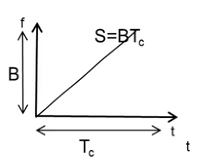
\includegraphics[width = .3\textwidth]{pic/problem_1.png}

}
解:\(\Delta f=\frac{S2\Delta d}{c};\Delta f>\frac{1}{T_c} \),其中$T_c$为IF信号的持续时间\\
请注意此处忽略FMCW一开始的线性调频脉冲的往返时间τ\\
则有:$\frac{S2\Delta d}{c}>\frac{1}{T_c}$\\
可得$\Delta d>\frac{c}{2ST_c}$,且斜率S*线性调频脉冲的持续时间$T_c$等于带宽B\\
∴$\Delta d>\frac{c}{2B},d_{res}=\frac{c}{2B}$\\
\subparagraph{问题二:}如下图所示,若两个雷达的带宽相同,而线性调频脉冲的持续时间不同,哪一个的距离分辨率更好?\\
{\centering 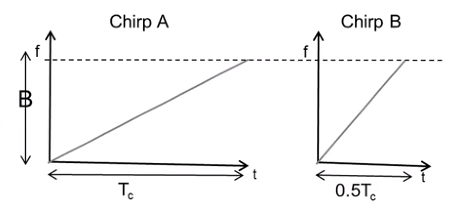
\includegraphics[width = .35\textwidth]{pic/problem_2.png}

}
解:根据问题一所得结果,他们应具有相同的距离分辨率。\\
但Chirp A具有更长的IF信号持续时间,因此具有更长的IF信号观测窗口。因此Chirp A的距离分辨率应优于Chirp B.与问题一矛盾。因此引出IF信号的数字化:
\subparagraph{IF信号的数字化:}有如下几条信息:\\
(1).我们所感兴趣的IF信号的带宽由我们想要的最大探测距离决定:\(f_{IF\_max}=\frac{S2d_{max}}{c}=\frac{2B}{c}\)\\
(2).IF信号通常首先经过低通滤波器,后经过ADC输入至DSP被处理\\
(3).IF带宽因此被ADC采样率$(F_s)$限制.\(F_s >= \frac{S2d_{max}}{c}\)\\
请注意:Nyquist采样定理限定了实信号的采样率应大于等于信号最大频率的2倍,但这里假设基带信号是复信号,因此上式Nyquist采样率为实信号的一半.\\
∴ADC采样率$F_s$限制了雷达的最大探测距离:\(d_{max}=\frac{F_sc}{2S}\)\\
结论:带宽与ADC采样率为影响雷达性能的瓶颈。\\
由于$d_{max}=\frac{F_sc}{2S}$,S与$d_{max}$成正比,可以权衡S与$d_{max}$,设计符合应用目的的雷达。\\
注意:通常雷达倾向于拥有更大的探测距离,因此具有更小的斜率S。

回到问题二上,由于A、B的带宽相同,则它们的距离分辨率相同。但由于Chirp A的斜率S小于Chirp B的斜率,因此对于相同的最大距离要求$d_{max}$,线性调频脉冲A仅需要一半的IF带宽,因此对其进行采样的ADC具有较小的采样率。因此Chirp A的测量时间较长;线性调频脉冲B仅需要一半的测量时间。
\subsubsection{提高mmWave性能方法}
\subparagraph{1:增大IF信号的长度$T_c$},即拓展两个正弦波的观测窗口。请思考这样做可以分开两个频率相近的正弦波信号的原因。请注意:增大观测窗口同时也潜在地增大了带宽,此带宽称为射频带宽(线性调频脉冲的带宽),其范围在几GHz到几百MHz之间。直观上即大带宽对应更好的分辨率。
\subparagraph{2:提高线性调频脉冲频域的斜率S}即增大IF带宽($f_{IF\_max}$),更大的IF带宽等效于更快的线性调频脉冲(即$T_c$更短),更大的最大探测距离$d_{max}$
%Module 2
\subsection{IF信号的相位}
\paragraph{}相位可以响应物体极小的位移,雷达正是基于此原理测量速度的变化。首先提醒一下:在傅里叶变换中,单正弦信号的频谱的峰值的相位对应于正弦波的初始相位。

{\centering 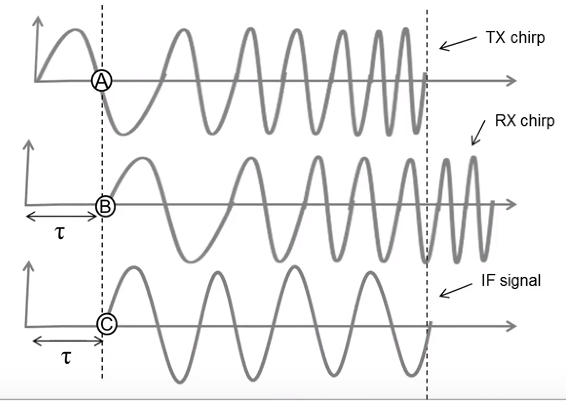
\includegraphics[width = .4\textwidth]{pic/phaseOfIF.png}

}
上图中IF信号为TX、RX经过混频器输出的信号$Asin(2\pi*ft+\phi_0)$,其中频率$f=\frac{S2d}{c}$
\subparagraph{IF信号的相位也会发生相应变化}$\phi_0$=$\phi_A+\phi_B$则当物体移动后,TX-RX发送接收延迟增加Δτ,则此时RX的相位不变,TX相位变化为($\phi_A+2\pi f_c\Delta\tau=\frac{4\pi \Delta d}{\lambda}$)等于IF相位变化。

{\centering 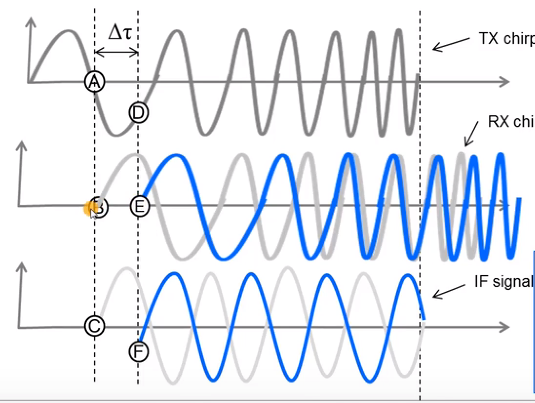
\includegraphics[width = .4\textwidth]{pic/phaseplustau.png}

}

结论:即:IF信号$Asin(2\pi*ft+\phi_0)$的频率随物体间距变化,其起始相位随物体距离的微小变化Δd成线性变化。此处的“微小变化”指相对于雷达的距离分辨率而言的。它必须为若干毫米。\\
\subsubsection{IF信号与物体微小位移的关系}
\paragraph{举例:} 
线性调频脉冲如下图。考虑当雷达前方的物体发生了1mm的位移时,IF信号的变化。(注:对77GHz雷达,1mm=$\lambda/4$)

{\centering 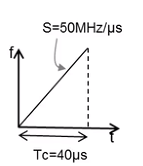
\includegraphics[width = .3\textwidth]{pic/IFsensitivity.png}

}

解:由前面推导:IF信号的相位变化$\Delta \phi=\frac{4 \pi \Delta d}{\lambda}=\pi=180^\circ$\\
IF信号的频率变化$\Delta f=\frac{S2\Delta d}{c}=333Hz$\\
对于观察窗口$T_c=40us$,$\Delta f$对应周期数目为$\Delta f T_c=333*40*10^-6=0.013 cycles$,如此微小的变化在FFT中体现不出来。\\
结论:IF信号的相位对物体距离的微小变化量十分敏感,而频率对其不敏感。
\subsubsection{用两个线性调频脉冲测量物体速度v}

{\centering 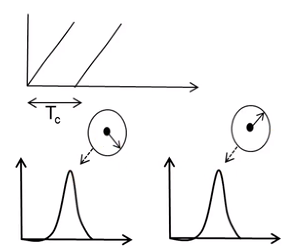
\includegraphics[width = .4\textwidth]{pic/speedmes.png}

}

\paragraph{}以$T_c$为时间间隔发送两个线性调频脉冲,对得到的IF信号进行FFT运算,他们将有相同的峰值但相位不同。测得的相位差$\omega$对应于物体的运动$vT_c$。\\
\[\omega=\frac{4\pi v T_c}{\lambda} ,v=\frac{\lambda \omega}{4\pi T_c}\]



由上式,可知$\Delta \phi$与$\Delta d$成正比,$\Delta \phi$的变化周期T也直接反映了震动周期。

{\centering 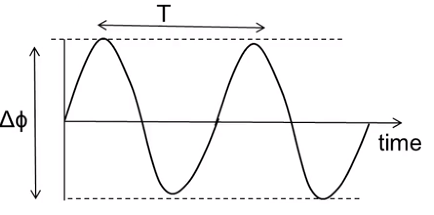
\includegraphics[width = .4\textwidth]{pic/deltaphase.png}

}

\subparagraph{补充}:\\
(1) 由于mmWave雷达对于微小振动敏感,因此也常用来作为电机振动监测、心跳检测等应用的核心部件。\\
(2) 当有多个物体恰好与雷达的距离相同,但拥有不同的移动速度。那么距离FFT(Range FFT,即上文中使用的FFT)将只输出单个与此距离d对应的峰值。分离方法:多普勒FFT:用于分离多个距离相同但速度不同的物体。
%Module 3
\subsection{速度估计}
\paragraph{FFT}
\end{document}